\documentclass[export, 12pt, letterpaper]{ctexrep}

\usepackage{titling}
\usepackage{standalone}
\usepackage{fontenc}


\usepackage[x11names]{xcolor}
\definecolor{SaddleBrown}{rgb}{0.55, 0.27, 0.07}
\definecolor{IndianRed}{rgb}{0.80, 0.36, 0.36}
\definecolor{Firebrick}{rgb}{0.70, 0.13, 0.13}
\definecolor{DarkBlue}{rgb}{0, 0, 0.55}
\definecolor{Goldenrod}{rgb}{0.85, 0.65, 0.13}
\definecolor{Peru}{rgb}{0.85, 0.65, 0.13}




\usepackage{hyperref}
\hypersetup{
    colorlinks=true,
    linkcolor=DarkBlue,
    urlcolor=blue,
    linktoc=all
}
\setcounter{tocdepth}{1}


\usepackage{mathtools}
\usepackage{amsmath}
\usepackage{tikz}
\usepackage{verbatim}
\usetikzlibrary{calc}

% put color to \boxed math command
\newcommand*{\boxcolor}{Peru}
\makeatletter
\renewcommand{\boxed}[1]{\textcolor{\boxcolor}{%
\tikz[baseline={([yshift=-1ex]current bounding box.center)}] \node [rectangle, minimum width=1ex,rounded corners,draw] {\normalcolor\m@th$\displaystyle#1$};}}
\makeatother


\usepackage{listings}

\definecolor{codegreen}{rgb}{0,0.6,0}
\definecolor{codegray}{rgb}{0.5,0.5,0.5}
\definecolor{codepurple}{rgb}{0.58,0,0.82}
\definecolor{backcolour}{rgb}{0.95,0.95,0.92}

\lstdefinestyle{mystyle}{
    backgroundcolor=\color{backcolour},
    commentstyle=\color{codegreen},
    keywordstyle=\color{magenta},
    numberstyle=\tiny\color{codegray},
    stringstyle=\color{codepurple},
    basicstyle=\ttfamily\footnotesize,
    breakatwhitespace=false,
    breaklines=true,
    captionpos=b,
    keepspaces=true,
    numbers=left,
    numbersep=5pt,
    showspaces=false,
    showstringspaces=false,
    showtabs=false,
    tabsize=2
}

\lstset{style=mystyle}


\usetikzlibrary{positioning}
\usetikzlibrary{petri} % LATEX and plain TEX
\usetikzlibrary[petri] % ConTEXt
\usepackage{pgfplots}
\pgfplotsset{compat=1.13}


\usepackage{framed}
\usepackage{quoting}

\colorlet{shadecolor}{LightSteelBlue1}
\usepackage{lipsum}
\newenvironment{shadedquotation}
 {\begin{shaded*}
  \quoting[leftmargin=5pt, rightmargin=5pt, vskip=0pt]
 }
 {\endquoting
 \end{shaded*}
}


\usepackage{lipsum} % for dummy text
\usepackage{enumitem}
\setlist{nosep} % or \setlist{noitemsep} to leave space around whole list


\usepackage{graphicx}
\usepackage{adjustbox}
\usepackage{caption}
\usepackage{float}

\pagestyle{plain}

\usepackage{ctex}
\usepackage{xeCJK}
\xeCJKsetup{CJKmath=true}


            \usepackage[
                left=1.0in,
                right=1.0in,
                top=1.5in,
                bottom=1.5in,
            ]{geometry}
        

\setlength{\droptitle}{-18em}
\title{\fontsize{40}{20} \textbf{\textcolor{red}{\kaishu README}}}
\author{\textcolor{red}{南方小智}}
\date{\textcolor{red}{\today}}



\begin{document}

\maketitle
\thispagestyle{empty}
\newpage

\setcounter{page}{1}
\tableofcontents
\newpage



\chapter{概述}


通过运行以下命令,可以将本Markdown文档生成pdf格式,建议阅读pdf版本的README。

\begin{lstlisting}[language=Bash]
make readme
\end{lstlisting}

本工具用于个人辅助写作和作图等,满足各种文档编辑的需求。


\begin{itemize}
\item{ 该系统写作部分以基本的Markdown语法为核心,作图部分使用Latex和dot等通用工具包。 }
\item{ 该系统会生成Markdown语法树,可通过Latex渲染生成pdf等,也可以通其他渲染方式生成Html,Word等格式,方便发布文章。 }
\item{ 该系统支持将批量的Markdown文档整理成册,比如合成一本书,并设置封面和章节目录等。 }
\item{ 该系统可以通过pgfplot,tikz等工具,快速制作复杂的数学图片。 }
\end{itemize}



\section{处理单个文档}
本系统可以将一个Markdown文档转化为tex文档,并自动生成封面和目录,后续还通过latex工具包转化为pdf。只需要将文档路径传入path。

\begin{lstlisting}[language=Bash]
python3 create_book.py --path README.md --name README --author 南方小智
@echo 'xelatex cmd support Chinese'
xelatex -output-directory log README.tex
@echo 'run twice to build toc correctly'
xelatex -output-directory log README.tex
\end{lstlisting}


\begin{itemize}
\item{ name代表生成的文件名和封面标题。 }
\item{ author代表生成的封面作者。 }
\item{ 生成的tex文件在log文件夹中。 }
\end{itemize}


\section{处理多个文档}
本系统可以将多个Markdown文档合成一个tex文档,并自动生成封面和目录,后续还通过latex工具包转化为pdf。只需要将所有文档放在同一个文件夹里,并将文件夹路径传入path。


\begin{lstlisting}[language=Bash]
python3 create_book.py --path examples/趣题集/ --name 趣题集 --bg images/趣题集/background.jpeg --author 南方小智
@echo 'xelatex cmd support Chinese'
xelatex -output-directory log 趣题集.tex
@echo 'run twice to build toc correctly'
xelatex -output-directory log 趣题集.tex
\end{lstlisting}


\begin{itemize}
\item{ 支持多层文件夹,每层文件夹对应一个目录级别,比如文件夹内第一层目录每个文件夹名字为每章的名字,第二层目录每个文件夹名字为每节的名字。 }
\item{ MAIN文件为保留文件名,为该层目录对应章节的导言部分。 }
\item{ \_INDEX文件为保留文件名,用于对文件夹(章节)进行排序,目前章节的排列方法是较长的章节放在靠前的位置。 }
\item{ 名字以“\_”开始的文件夹或者文件会被忽略。 }
\end{itemize}


\_INDEX文件中按顺序列举该层目录的标题,未列举的标题将放在“*”的位置。如果“*”未标注在文件中,则未列举的标题默认排到最后。

\lstinputlisting[language=]{examples/趣题集/_INDEX}


\section{生成图片文件}
本系统可以编译单一tex文档,并生成图片。只需要使用simple参数,就可以省略标题,目录,页码等,生成一个独立的图片形式,后续可以用convert命令将pdf转为图片。

\begin{lstlisting}[language=Bash]
python3 create_book.py --path images/趣题集/三角形悖论/image0.tex --name 三角形 --simple
xelatex -output-directory log 三角形.tex
@echo '需要安装brew install imagemagick'
convert -density 300 log/三角形.pdf -quality 90 log/三角形.png
\end{lstlisting}

\section{所有测试用例}
\begin{lstlisting}[language=Bash]
make readme     # 将本文档生成pdf
make all        # 生成一本《趣题集》
make image      # 生成一张png图片 (需要安装brew install imagemagick)
make clean      # 清空log文件
make clean_all  # 清空所有生成文件,包括,log文件,tex文件, pdf文件等
\end{lstlisting}

具体细节请参照makefile:

\lstinputlisting[language=Bash]{makefile}

\chapter{Markdown支持}

基本语法请参照:\href{https://simplemde.com/markdown-guide}{markdown wiki}

\section{特殊字符}

在Markdown文件中使用特殊字符时需要进行特殊处理,比如添加转义字符$\backslash$
\begin{lstlisting}[language=Bash]
_ -> \_   # _ 在Markdown中可用于表示斜体
* -> \*   # * 在Markdown中可用于表示斜体
$ -> \$   # $ 在Markdown中可用于开始数学表达式模式
\ -> \\   # \ 是特殊的Latex符号
\end{lstlisting}

\section{导入代码文件}

\begin{lstlisting}[language=Bash]
{{create_book.py}}[code:Python] # 导入Python格式的代码文件
\end{lstlisting}

\lstinputlisting[language=Python]{create_book.py}

\section{导入tex格式的图片文件}

\begin{lstlisting}[language=Bash]
{{images/趣题集/三角形悖论/image1.tex}}[image] # 导入tex格式的图片文件
\end{lstlisting}

\begin{center}
\begin{tikzpicture}
\coordinate [label=above:\textcolor{red}{$A$}] (A) at (0.5,4);
\coordinate [label=left:\textcolor{red}{$B$}] (B) at (-2,0);
\coordinate [label=right:\textcolor{red}{$C$}] (C) at (2,0);
\coordinate [label=right:\textcolor{black}{$O$}] (O) at (0,1);

\coordinate [label=below:\textcolor{blue}{$A'$}] (A_1) at (0,0);

\draw[black, thick] (A) -- (B) node(A_B_line)[] {};
\draw[black, thick] (B) -- (C);
\draw[black, thick] (C) -- (A);
\draw[black, thick] (O) -- (A_1);
\draw[black, thick, dotted] (O) -- (B);
\draw[black, thick, dotted] (O) -- (C);
\draw[black, thick] (O) -- (A);


\draw[black, thick, dotted] (O) -- ($(A)!(O)!(B)$) node(C_1)[label=left:\textcolor{blue}{$C'$}] {};
\draw[black, thick, dotted] (O) -- ($(A)!(O)!(C)$) node(B_1)[label=right:\textcolor{blue}{$B'$}] {};

\foreach \point in {A,B,C, O}
\fill [black,opacity=.8] (\point) circle (2pt);

\foreach \point in {A_1, B_1, C_1}
\fill [black,opacity=.5] (\point) circle (2pt);


\end{tikzpicture}

\end{center}


\section{导入dot格式的图片文件}

\begin{shadedquotation}
\noindent
注意:需要安装\href{https://graphviz.org/download/}{Graphviz}。
\end{shadedquotation}


导入的dot文件会通过dot命令转化为eps格式,并作为图片导入到tex文件中。dot的简单用法可以参照\href{https://graphviz.org/documentation/}{GraphViz Documentation}。

\begin{lstlisting}[language=Bash]
{{images/README/image0.dot}}[dot:测试dot] # 导入dot格式/graphviz语法的图片文件,并用“测试dot”作为标题。
\end{lstlisting}

\begin{center}\begin{figure}[H] \centering 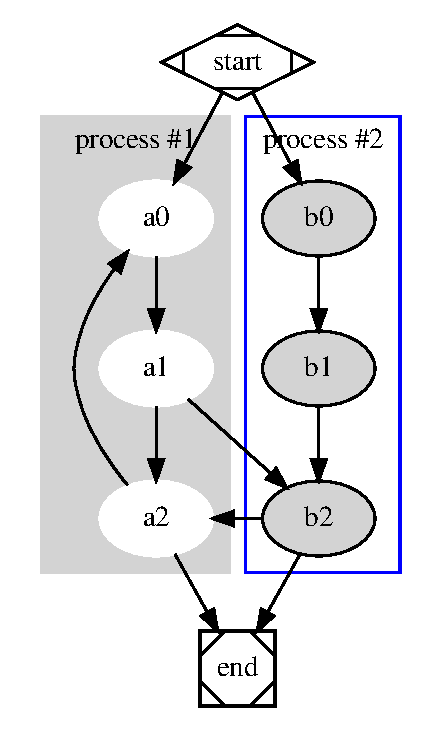
\includegraphics[max size={\textwidth}{\textheight},keepaspectratio]
{images/README/image0.dot.eps}\caption*{测试dot}
\end{figure} \end{center}


\section{Markdown的解析和渲染}
该系统自带一个Markdown解析器,会将Markdown文本转化为一棵语法树。使用如下命令可以打印出本Readme文档的语法树:

\begin{lstlisting}[language=Bash]
make test  # python3 test.py --path README.md
\end{lstlisting}

Markdown语法树的解析遵循如图的树状结构。从最顶端的Document到最底端的Line,而inline部分的语法则较为简单,将由渲染器进行解析。
\begin{center}\begin{figure}[H] \centering 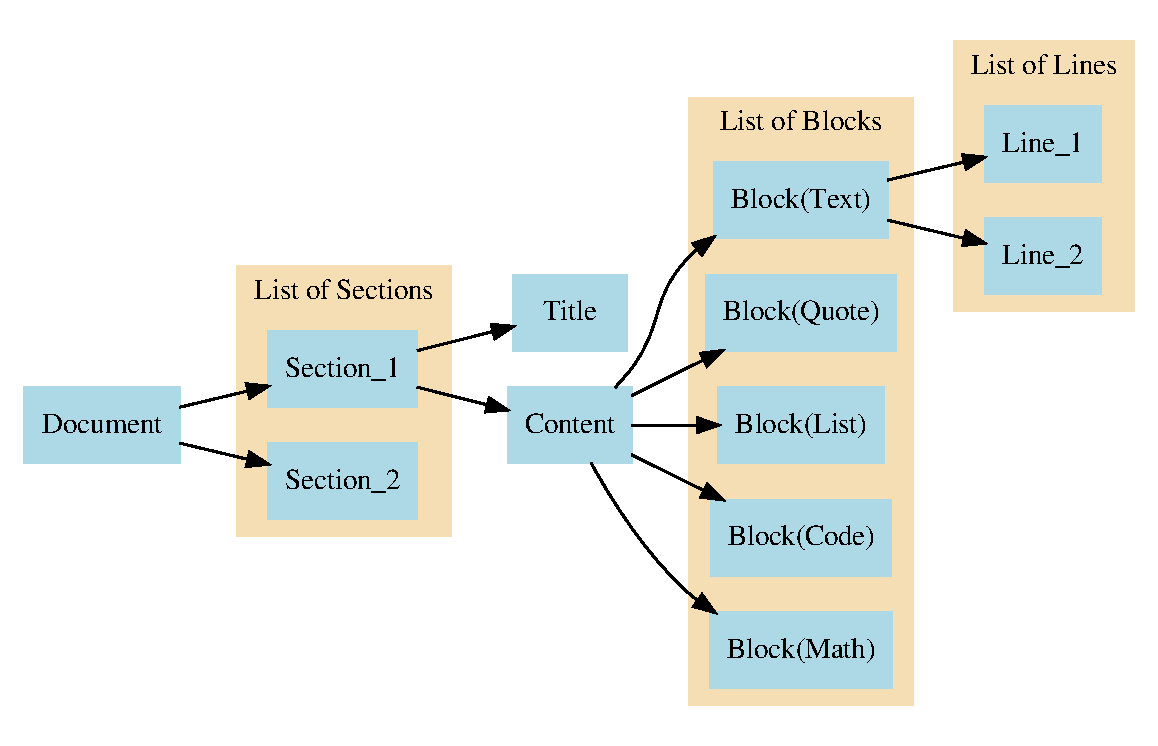
\includegraphics[max size={\textwidth}{\textheight},keepaspectratio]
{images/README/image1.dot.eps}\caption*{Markdown语法树}
\end{figure} \end{center}

通过渲染器,可以将Markdown渲染成tex,html,word等格式。只需要继承MDRender,实现对应的抽象方法即可添加新的渲染器,比如src/render/md\_tex\_render.py。

\lstinputlisting[language=Python]{src/render/md_render.py}


\chapter{TODO}


\begin{itemize}
\item{ 目前很多latex设置都是Hard Code的,应当将这些设置变成可配置的:
\begin{itemize}
\item{ 目前目录最多显示两层标题结构 }
\item{ 目前最高层目录默认为Chapter,设置level参数使其可配置化 }
\item{ 图片默认居中,可以考虑配置化。 }
\end{itemize}
 }
\item{ 目前Markdown解析器仍然有许多Markdown基本语法并不支持,需要:
\begin{itemize}
\item{ 支持行内斜体,下划线等。 }
\item{ 支持行内代码。 }
\item{ [Done] 支持一般图片格式的导入。 }
\item{ [Done] 支持嵌套List。
\begin{itemize}
\item{ 测试3层嵌套。 }
\end{itemize}
 }
\item{ 支持表格 }
\end{itemize}
 }
\item{ 目前Latex渲染器仍然有一些Latex用法支持不够,需要:
\begin{itemize}
\item{ 支持更多类似\$,$<$,$>$等latex特殊字符。 }
\end{itemize}
 }
\item{ 支持更多的Features:
\begin{itemize}
\item{ 使用folder模式的时候,兼容.md等后缀。 }
\item{ 添加页面背景水印,这样可以防止发布的材料被盗版使用。 }
\item{ 添加程序辅助画图(特别是制作复杂的各类数学图片)。 }
\item{ 添加作者介绍。 }
\item{ 添加html和word渲染器。 }
\item{ 支持latex画思维导图。 }
\end{itemize}
 }
\item{ BUG:
\begin{itemize}
\item{ tex图片嵌入应该像dot图片嵌入一样支持设置标题,如[image:title]。 }
\end{itemize}
 }
\item{ Better Engineering:
\begin{itemize}
\item{ md\_tree的Parser主体可以用自动机的方式实现,从而减少if/else的判断和重复代码片。 }
\end{itemize}
 }
\end{itemize}


\begin{center}\begin{figure}[H] \centering 
\includegraphics[max size={\textwidth}{\textheight},keepaspectratio]
{images/README/qrcode_for_haqiandahulu_m_size.jpg}\caption*{扫码支持作者}
\end{figure} \end{center}

\end{document}
